
\section{Lumped and Distributed Element Models}
\subsection{Tunable Coupler}
Here we will look at a simulation of a system containing a tunable coupler \cite{tunable_coupler} to explicitly see where the approximations of Section \ref{section:effective_coupling} start to break down. Specifically, we want to see what happens to the estimate for the effective coupling rate (\ref{eq:eff_qubit_coupling}) when the coupler approaches the qubit frequency such that $g/\Delta \centernot{\ll} 1$. Note that since this system only contains two qubits and a coupler, (\ref{eq:eff_qubit_coupling}) reduces to the result for the effective coupling rate from \cite{tunable_coupler}.

In Fig.\ \ref{fig:tc_circuit}, we see a circuit that contains 3 transmon qubits. The two outer qubits are used as computational qubits and the center one is used as a coupler. Since the network is purely capacitive apart from the junctions, the circuit Hamiltonian can easily be found and is of the form (\ref{eq:transmon_resonator_ham}) with only transmon branches. With the circuit Hamiltonian, we can simulate the time evolution of the system. The results of the simulation can then be compared to the effective coupling rates.

\begin{figure}[h!]
    \centering
    \begin{circuitikz}[line width=1pt]
        \ctikzset{bipoles/thickness=1, bipoles/length=1cm, monopoles/ground/thickness=0.75}
        \ctikzset { label/align = straight }

        % ---------------------------------- Coupler --------------------------------- %
        \draw (0,0) -- (0,-0.5) -- (-0.5,-0.5) to[C,l_=$C_c$] (-0.5,-1.5) -- (0,-1.5);
        \draw (0,-0.5) -- (0.5,-0.5) to[barrier=$E_{J_c}$, label distance=-10pt] (0.5,-1.5) -- (0,-1.5);
        \draw (0,-1.5) -- (0,-1.55) node[ground] {};

        % -------------------------------- Transmon 1 -------------------------------- %        
        \draw (-3,0) -- (-3,-0.5) -- (-3.5,-0.5) to[C,l_=$C_1$] (-3.5,-1.5) -- (-3,-1.5);
        \draw (-3,-0.5) -- (-2.5,-0.5) to[barrier=$E_{J_1}$, label distance=-10pt] (-2.5,-1.5) -- (-3,-1.5);
        \draw (-3,-1.5) -- (-3,-1.55) node[ground] {};

        % -------------------------------- Transmon 2 -------------------------------- %
        \draw (3,0) -- (3,-0.5) -- (2.5,-0.5) to[C,l_=$C_2$] (2.5,-1.5) -- (3,-1.5);
        \draw (3,-0.5) -- (3.5,-0.5) to[barrier=$E_{J_2}$, label distance=-10pt] (3.5,-1.5) -- (3,-1.5);
        \draw (3,-1.5) -- (3,-1.55) node[ground] {};

        % ---------------------------- Capacitive Coupling --------------------------- %
        \draw (-3,0) to[C=$C_{1c}$] (0,0) to[C=$C_{2c}$] (3,0);
        \draw (-3,0) -- (-3,1) to[C=$C_{12}$] (3,1) -- (3,0);

    \end{circuitikz}
    \caption{Model for the circuit implementing a tunable coupler (center transmon) to control the coupling between the two outer transmons. The circuit parameters we use are also used in the example given in \cite{tunable_coupler}: $C_1=$ 70 fF, $C_2=$ 72 fF, $C_c=$ 200 fF, $C_{1c}=$ 4 fF, $C_{2c}=$ 4.2 fF, $C_{12}=$ 0.1 fF. In the simulations, we treat each of the three Josephson junctions as tunable.}
    \label{fig:tc_circuit}
\end{figure}

To simulate the time evolution of the tunable coupler system, we will use \texttt{sesolve} from QuTiP \cite{qutip1,qutip2} for the Hamiltonian (\ref{eq:transmon_resonator_ham}) of the circuit in Fig.\ \ref{fig:tc_circuit}. For the transmons, we use three level systems. We represent the system state using the notation $\ket{Q_1,Q_c,Q_2}$ where $Q_{1/2}$ correspond to the computational qubits and $Q_c$ to the coupler state. By initializing the system in state $\ket{100}$ and putting the states $\ket{100}$ and $\ket{001}$ on resonance, we see oscillations in the $\ket{001}$ state population from which we can extract the coupling rate. Doing this while sweeping over the coupler frequency, we obtain the results in Fig.\ \ref{fig:tc_time_evolution}.

To extract the effective coupling rates between the two computational qubits from the simulation, we can fit the oscillations in the $\ket{001}$ population. The fitted coupling rates can then be compared to the estimate of the effective coupling rate from (\ref{eq:eff_qubit_coupling}). The results of this comparison are shown in Fig.\ \ref{fig:eff_vs_sim_coupling}. We can see that the effective coupling rates start to stray away from the theoretical estimate as the coupler gets closer to the computational transmon frequencies. In this case, the deviation is over 1 MHz once $g_{1c}/\Delta_{1c} \approx  -0.3$, and is increasing as the coupler frequency gets lower. This is to be expected, since $g_{1c}/\Delta_{1c} \centernot{\ll} 1$ and the system is approaching the nondispersive regime where the couplings can no longer be treated as perturbations. We see that when the coupler is far from the qubit frequencies, the approximation is much better. Thus, when using the formulas for the effective coupling rates, we need to take care that we are in the dispersive regime with $g \ll \Delta$. This is especially relevant in systems with tunable qubits and couplers since $g$ and $\Delta$ will depend on these frequencies. 

\begin{figure}[!h]
    \centering
    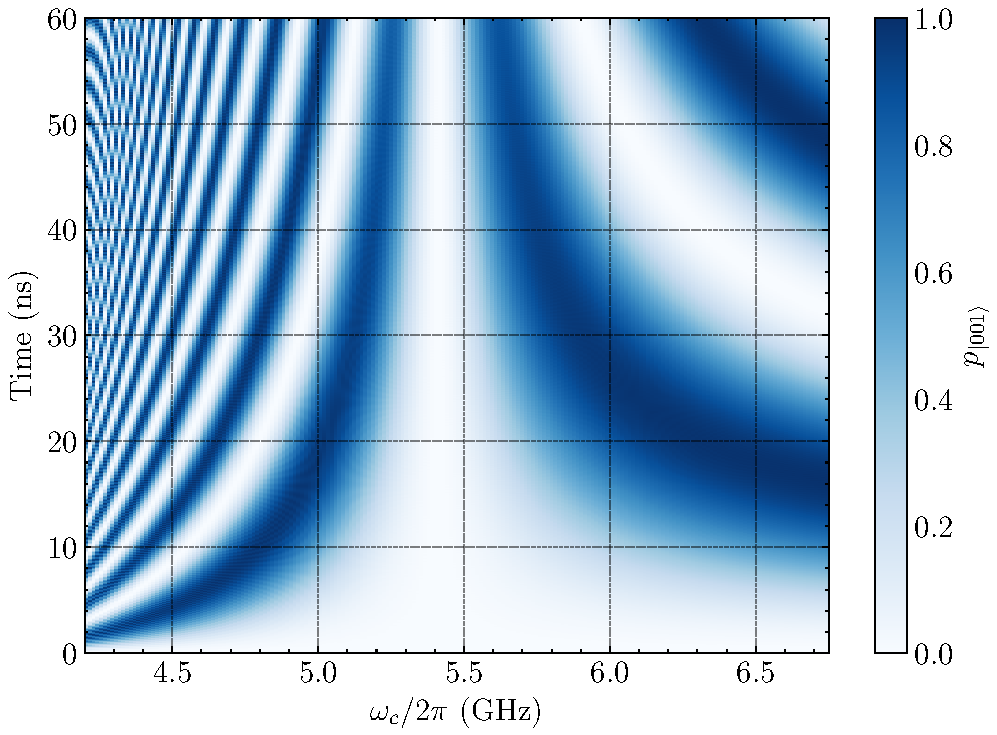
\includegraphics[width=.75\textwidth]{figures/TC_time_evolution.pdf}
    \caption{Time simulation results for the tunable coupler system in shown in Fig.\ \ref{fig:tc_circuit}. The system is initialized in state $\ket{100}$ and the two computational transmons are put on resonance such that $\omega_1/2\pi=\omega_2/2\pi=4$ GHz. The resulting oscillations in the population of state $\ket{001}$ are plotted above for various coupler frequencies.}
    \label{fig:tc_time_evolution}
\end{figure}

\begin{figure}[!h]
    \centering
    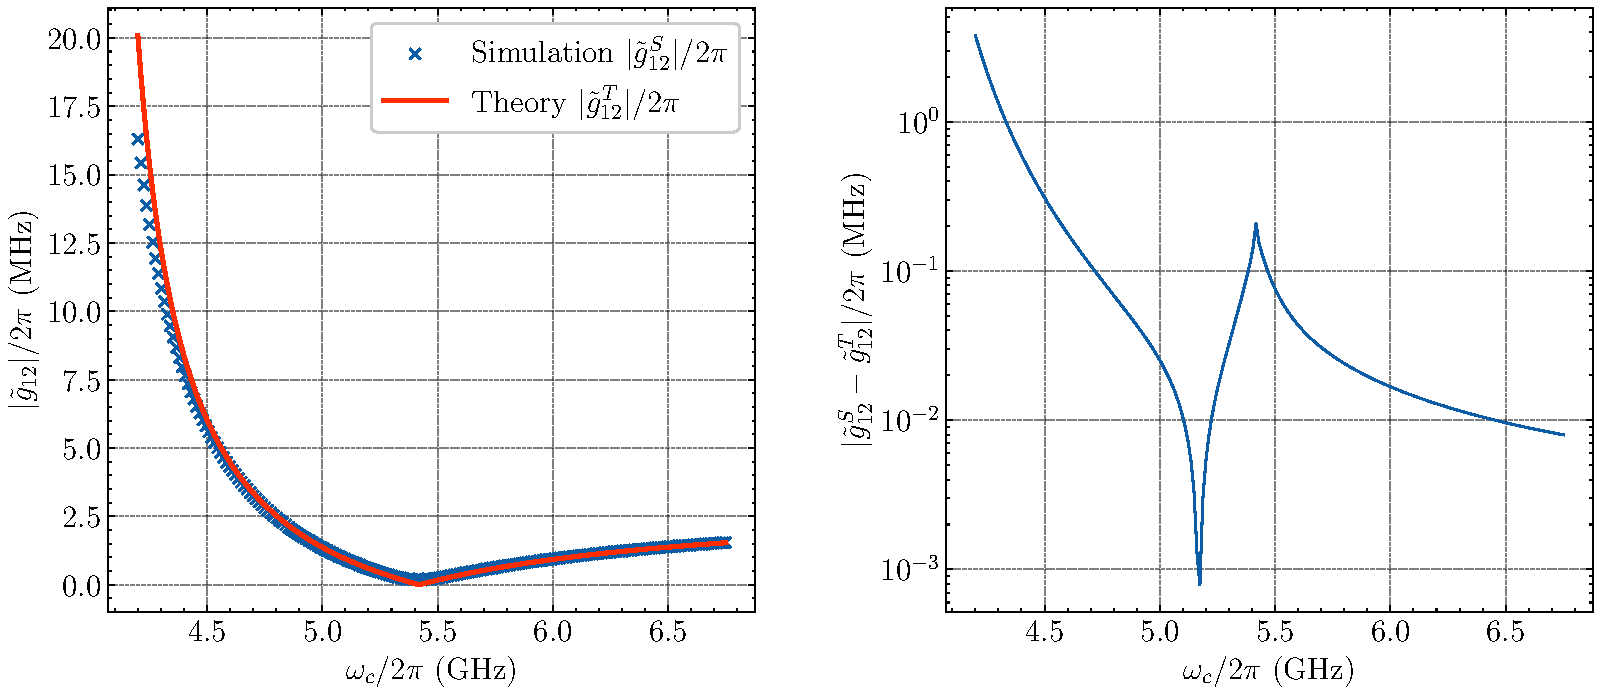
\includegraphics[width=\textwidth]{figures/TC_sim_th_eff_coupling.pdf}
    \caption{Left: Comparison between the theoretical and fitted effective coupling from the simulation in Fig.\ \ref{fig:tc_time_evolution}. Right: Difference between the theoretical and effective coupling extracted from the simulation.}
    \label{fig:eff_vs_sim_coupling}
\end{figure}

When attempting to implement fast two qubit gates in the nondispersive regime, leakage into the coupler can occur due to its higher participation in the coupling compared to the dispersive regime. An example of this is shown in Fig.\ \ref{fig:tc_time_evolve_example}. Nonetheless, the potential leakage to the coupler and higher energy levels during gate operations can be suppressed by control pulse optimization, which allows for fast gates to be implemented \cite{high_fidelity_cz_iswap_tc}. However, as we've seen, the formulas for the effective coupling rates (\ref{eq:eff_qubit_coupling}) will not be accurate in this regime. While not accurate in the nondispersive regime, the formulas can still provide a good estimate for the point at which the effective coupling is ``off''.

\begin{figure}[!h]
    \centering
    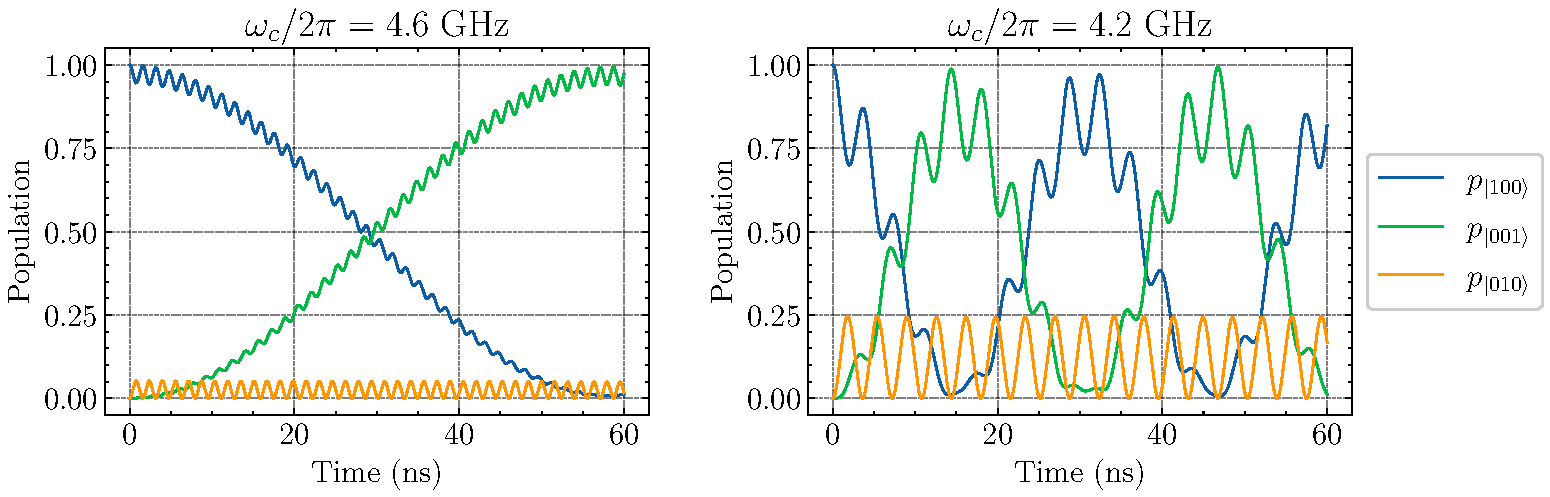
\includegraphics[width=\textwidth]{figures/TC_time_evolution_examples.pdf}
    \caption{Time evolution of state populations for circuit \ref{fig:tc_circuit} and $\omega_1/2\pi=\omega_2/2\pi=4$ GHz and two different coupler frequencies. On the left, for the higher coupler frequency, $g_{1c}/\Delta_{1c} \approx -0.12$. On the right, we have $g_{1c}/\Delta_{1c} \approx -0.345$.}
    \label{fig:tc_time_evolve_example}
\end{figure}


\subsection{Qubit Decay Rates}\label{section:decay_rate_example}
We will now see how the results of Section \ref{section:ext_ports_decay} can be applied to a lumped element circuit containing two coupled qubits and four external ports. We will also use the example circuit to demonstrate that (\ref{eq:qubit_decay_admittance}) can provide a good approximation to the qubit decay rates.

\begin{figure}[h!]
    \centering
    \begin{circuitikz}[line width=1pt]
        \normalfont
        \ctikzset{bipoles/thickness=1, bipoles/length=.75cm, monopoles/ground/thickness=0.65}
        \ctikzset { label/align = straight }

        % -------------------------------- Transmon 1 -------------------------------- %
        \draw (-2.8,0) to[C,l_=$C_{J_1}$] (-2.8,-1);
        \draw[color=nodecolor] (-2.2,0) to[barrier=$E_{J_1}$, label distance=-10pt] (-2.2,-1);

        % -------------------------------- Transmon 2 -------------------------------- %
        \draw (2.2,0) to[C,l_=$C_{J_2}$] (2.2,-1);
        \draw[color=nodecolor] (2.8,0) to[barrier=$E_{J_2}$, label distance=-10pt] (2.8,-1);

        % ------------------------ Top and bottom lines across ----------------------- %
        \draw (0,0) -- (0.75,0) to[C=$C_r$] (1.75,0) -- (3.25,0) to[C=$C_r$] (4.25,0) -- (5.75,0) to[C=$C_{r}$] (6.75,0) to[short, -o] (8,0);
        \draw (-8,0) to[short, o-] (-6.75,0) to[C=$C_{r}$] (-5.75,0) -- (-4.25,0) to[C=$C_r$] (-3.25,0) -- (-1.75,0) to[C=$C_r$] (-0.75,0) -- (0,0);
        \draw (-8,-1) to[short, o-] (0,-1) to[short,-o] (8,-1);
        \draw (0,-1) -- (-0,-1.05) node[ground] {};

        % ---------------------------------- Coupler --------------------------------- %
        \draw (-0.3,0) to[C,l_=$C_c$] (-0.3,-1);
        \draw (0.3,0) to[L=$L_c$] (0.3,-1);

        % ----------------------- Transmon 1 Readout Resonator ----------------------- %
        \draw (-5.3,0) to[C,l_=$C_c$] (-5.3,-1);
        \draw (-4.7,0) to[L=$L_{R_1}$] (-4.7,-1);

        % ----------------------- Transmon 2 Readout Resonator ----------------------- %
        \draw (4.7,0) to[C,l_=$C_c$] (4.7,-1);
        \draw (5.3,0) to[L=$L_{R_2}$] (5.3,-1);

        % ----------------------- Readout Port Shunt Capacitors ---------------------- %
        \draw (-7.25,0) to[C=$C_s$] (-7.25,-1);
        \draw (7.25,0) to[C,l_=$C_s$] (7.25,-1);

        % -------------------------------- Drive Ports ------------------------------- %
        \draw (-2.5,0) -- (-2.5,2) to[C,l_=$C_d$] (-4.5,2) to[short, -o] (-5.5,2);
        \draw (-4.5,2) to[C=$C_s$] (-4.5,1) to[short,-o] (-5.5,1);
        \draw (-4.5,1) -- (-4.5,.95) node[ground] {};

        \draw (2.5,0) -- (2.5,2) to[C,l=$C_d$] (4.5,2) to[short, -o] (5.5,2);
        \draw (4.5,2) to[C,l_=$C_s$] (4.5,1) to[short,-o] (5.5,1);
        \draw (4.5,1) -- (4.5,.95) node[ground] {};

    \end{circuitikz}
    \caption{Circuit model for two resonator-coupled transmons where each is individually coupled to an external drive port and readout resonator. Overall, there are four external ports, two for drive, and two for readout. When discussing this circuit, we sometimes refer to the two transmon or qubit ports that are located at the positions of the Josephson junctions (marked in red). Transmons 1 and 2 have the Josephson energies $E_{J_1}$ and $E_{J_2}$, respectively. The values of the circuit elements are as follows: $C_{J_1}=$ 70 fF, $C_{J_1}=$ 75 fF, $C_s=$ 100 fF, $C_c=$ 300 fF, $C_r=$ 10 fF, $C_d=$ 0.15 fF, $L_c=$ 3.25 nH, $L_{R_1}=$ 2.1 nH, and $L_{R_2}=$ 1.6 nH. The external ports are assumed to have characteristic impedances of $Z_0=$ 50 $\Omega$.}
    \label{fig:decay_lumped_circuit}
\end{figure}

We consider the circuit in Fig. \ref{fig:decay_lumped_circuit}. If we fix the qubit inductances, we can find the eigenvalues of the matrix in (\ref{eq:matrix_eoms}) to obtain the complex poles that correspond to the resonant modes in the circuit. From these eigenvalues, we find two complex conjugate pairs that correspond to the transmon oscillator modes. Three other complex conjugate pairs are also found for the other resonant modes in the circuit. Now, we want to verify that these complex numbers are the complex poles of the impedance function for the circuit in Fig.\ \ref{fig:decay_lumped_circuit} with the external ports shunted by resistors and the transmon ports shunted by inductors (as shown in Fig.\ \ref{fig:lossy_transmon_network}). To compute the shunted impedance function at an arbitrary complex frequency, we first compute the impedance function for the circuit Fig.\ \ref{fig:decay_lumped_circuit} using the method of Section \ref{section:cascade_analysis}. Then we shunt the qubit ports with inductors and the external ports with resistors using (\ref{eq:cascade_s}). We find that the predicted pole locations from (\ref{eq:matrix_eoms}) match the positions of the poles of the lossy impedance function. This alignment is shown for one of the transmon poles in Fig.\ \ref{fig:shunted_impedance_plot}.

\begin{figure}[!h]
    \centering
    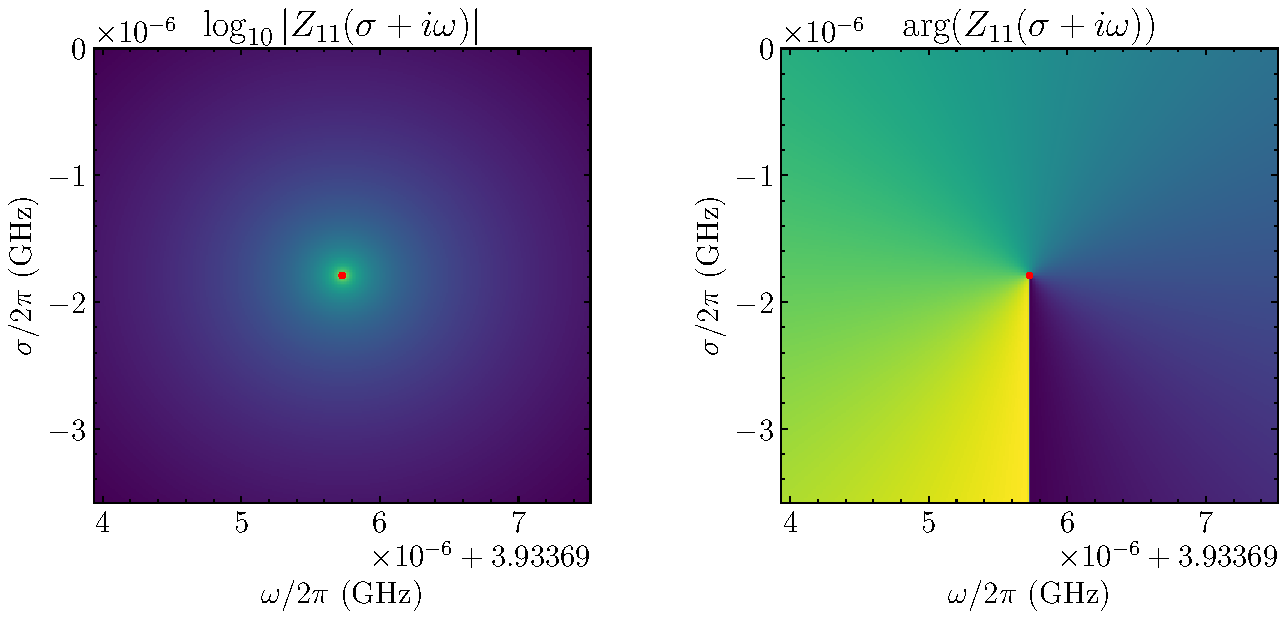
\includegraphics[width=\textwidth]{figures/fully_shunted_impedance.pdf}
    \caption{These plots show the magnitude and phase of the impedance function for the circuit in Fig.\ \ref{fig:decay_lumped_circuit} with inductors and resistors shunting the transmon and external ports, respectively. We have chosen $L_{J_1}=$ 18 nH and $L_{J_2}=$ 15.5 nH. In the plot, we look at a region around a complex pole that corresponds to transmon 1 in the circuit. We find that the predicted pole position computed by diagonalizing (\ref{eq:matrix_eoms}) aligns with the pole position in the numerically computed impedance.}
    \label{fig:shunted_impedance_plot}
\end{figure}

We have shown that diagonalizing (\ref{eq:matrix_eoms}) does in fact provide us with the complex poles of the shunted impedance function for a network of the form shown in Fig.\ \ref{fig:lossy_transmon_network}. With the complex pole positions, we can estimate the decay rate for a given resonant frequency using (\ref{eq:lossy_pole}). We can use this to compute the decay rates of the transmons at various frequencies by varying one of the transmon inductances and computing the poles for each inductance value. As an example, we do this for transmon 1 in the circuit, and the decay rates and resonant modes for all the computed poles are plotted in Fig.\ \ref{fig:poles_real_imag}. In these plots, we can see how the resonance frequency and decay rate of the transmon oscillator changes as the shunt inductance is changed.

Taking this method further, we can then see the relationship between the transmon resonant frequency and its relaxation time $T_1 = \kappa^{-1}$. We compare this to the qubit decay rate estimate using the admittance of the lossy network (\ref{eq:qubit_decay_admittance}). For the admittance, we can also choose to include or exclude the transmon inductances. We do this for both qubits and the results of the three methods are shown in Fig.\ \ref{fig:transmons_T1}. When plotting the poles computed from (\ref{eq:matrix_eoms}), there are peaks in the transmon lifetimes that are present due to the avoided level crossings shown in Fig.\ \ref{fig:poles_real_imag}. At the resonance crossings, the transmon oscillator is not well defined on its own, and thus the peaks should not be thought of as an expected point where the transmon lifetime is increased. In the plot using the admittance with ports shunted by inductors and resistors, there are sharp dips present that are not seen when only shunting with resistors. These dips are present because of the additional resonance mode of the other transmon. Comparing the methods, we see that using the admittance estimates can provide a good lower bound on the transmon relaxation times. We can also show that if we increase the coupling complexity of the network, this is still the case. We show this by adding a 1 fF capacitance between every node where one is not already present for the circuit in Fig.\ \ref{fig:decay_lumped_circuit}. The results for the relaxation time estimates for this new network are shown in Fig.\ \ref{fig:transmons_T1_ata}.

\begin{figure}[!h]
    \centering
    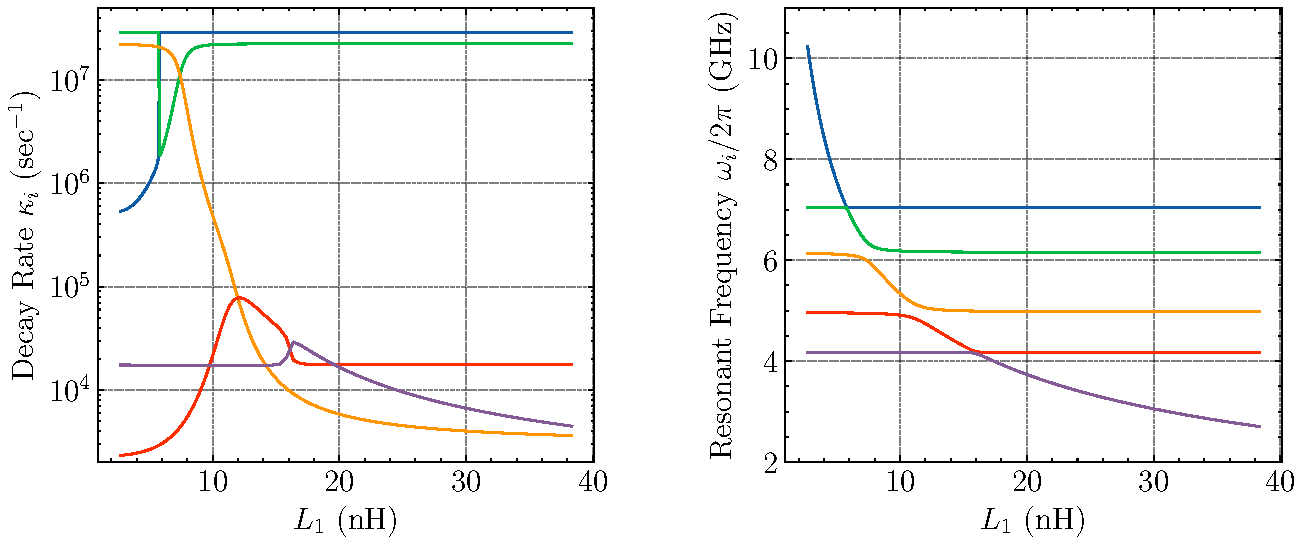
\includegraphics[width=\textwidth]{figures/poles_real_imag.pdf}
    \caption{Decay rates and resonant frequencies of the complex poles found by diagonalizing the matrix in (\ref{eq:matrix_eoms}) while varying the inductance shunting transmon 1. The inductance of transmon 2 is fixed at $L_{J_2}=$ 13.8 nH.}
    \label{fig:poles_real_imag}
\end{figure}

\begin{figure}[!h]
    \centering
    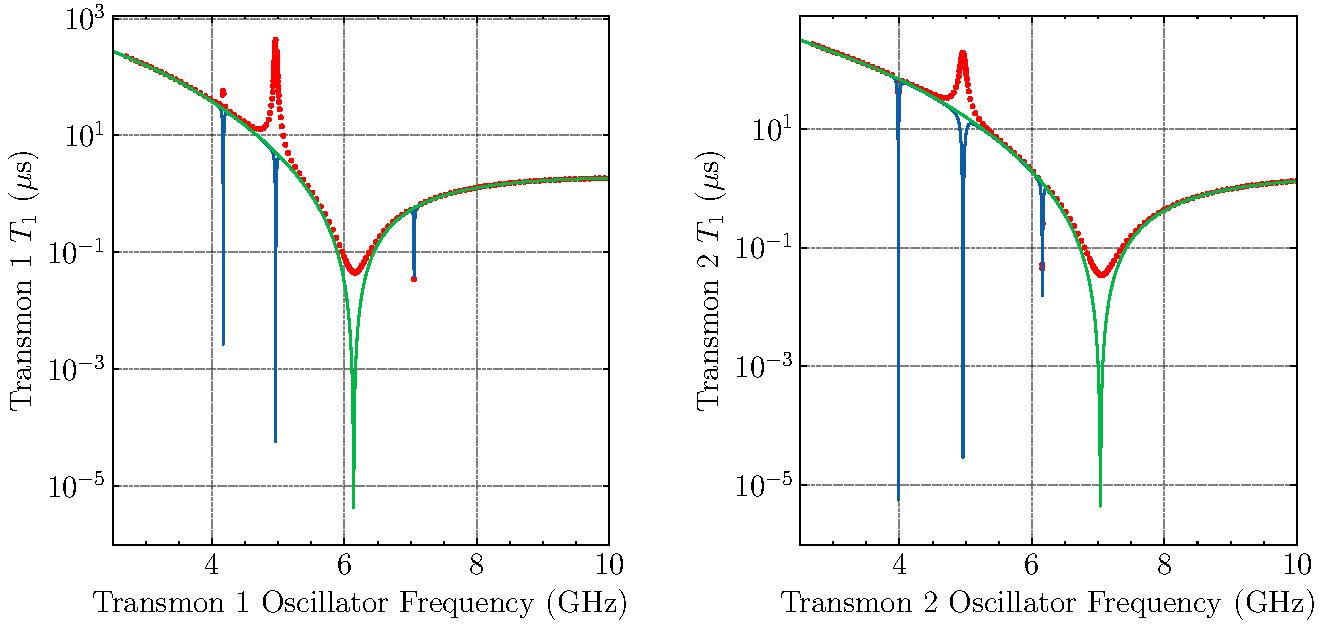
\includegraphics[width=\textwidth]{figures/lumped_transmons_T1.pdf}
    \caption{Above, we use three methods to plot estimates of the $T_1$ time of transmons 1 and 2 for the circuit in Fig.\ \ref{fig:decay_lumped_circuit}. \textbf{Red points:} The positions of the complex poles of the network found by diagonalizing the matrix in (\ref{eq:matrix_eoms}). As one transmon inductance is varied, the other is fixed. In the left plot, $L_{J_2}=$ 15.2 nH and on the right, $L_{J_1} =$ 17.5 nH. \textbf{Blue line:} $\Gamma_i^{-1}$ computed using the admittance in (\ref{eq:qubit_decay_admittance}) with the transmon ports shunted with inductors and the external ports shunted with resistors. \textbf{Green line:} Also using (\ref{eq:qubit_decay_admittance}), but the admittance is only shunted with resistors at the external ports.}
    \label{fig:transmons_T1}
\end{figure}

\clearpage
\begin{figure}[!h]
    \centering
    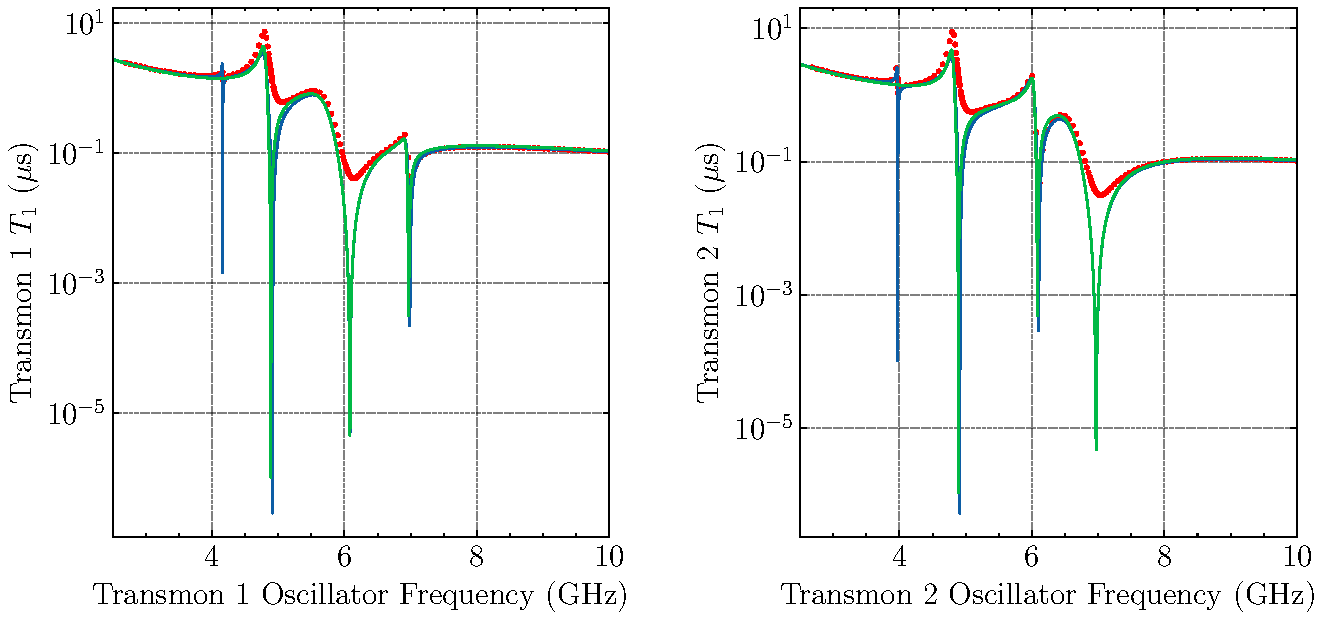
\includegraphics[width=\textwidth]{figures/lumped_transmons_T1_all_to_all.pdf}
    \caption{Same as Fig.\ \ref{fig:transmons_T1} except now there is an added 1 fF capacitance between nodes where there was no coupling present for the circuit in Fig.\ \ref{fig:decay_lumped_circuit}.}
    \label{fig:transmons_T1_ata}
\end{figure}

\subsection{Ideal Transmission Line Coupler}
Here, we consider a network of two qubits coupled by an ideal transmission line as shown in Fig.\ \ref{fig:ideal_TL_coupler}. Now we go through the process of obtaining the Hamiltonian from the impedance function of this two-port network.

\begin{figure}[h!]
    \centering
    \begin{circuitikz}[line width=1pt]
    \ctikzset{american}
    \ctikzset{bipoles/thickness=1, bipoles/length=1cm}
    \ctikzset{bipoles/crossing/size=0.5}
    \ctikzset { label/align = straight }

    \draw[color=nodecolor] (-2.5,1) -- (-3,1) to[barrier=$E_{J_1}$, label distance=-10pt]  (-3,-0.5) -- (-2.5,-0.5);
    \draw[color=nodecolor] (11,1) -- (11.5,1) to[barrier,l_=$E_{J_2}$, label distance=-10pt]  (11.5,-0.5) -- (11,-0.5);
    
    \draw (-2.5,1) to[short,o-] (0,1) to[short, o-] (0.5,1) to[C=$C_{1c}$] (2,1) to[short, -o] (2.5,1) to[short,-o] (6,1) -- (6.5,1) to[C=$C_{2c}$] (8,1) to[short, -o] (8.5,1) to[short, -o] (11,1);
    \draw (-2.5,-0.5) to[short,o-] (0,-.5) to[short,o-] (0.5,-.5) to[short, -o] (2.5,-.5) to[short, -o] (6,-.5) to[short,-o] (8.5,-.5) to[short, -o] (11,-0.5);

    \draw (-1.25,1) to[C=$C_1$] (-1.25,-0.5);
    \draw (9.75,1) to[C,l_=$C_2$] (9.75,-0.5);
    

    \node at (4.25,0.25) {$Z_0,\; \beta=\omega\sqrt{LC}$};
    
    \node at (4.25,-0.75) {$\ell$};
    \draw [-stealth](4.5,-0.75) -- (6,-0.75);
    \draw [-stealth](4,-0.75) -- (2.5,-0.75);

    \end{circuitikz}
    \caption{Two qubit circuit containing two transmon qubits coupled by an ideal transmission line. The network can be viewed as a two-port system shunted with two Josephson junctions.}
    \label{fig:ideal_TL_coupler}
\end{figure}

We can compute the two-port impedance function over a discretized frequency range by using ABCD matrices \cite[Chapter 4.4]{Pozar_2011}. The network in Fig.\ \ref{fig:ideal_TL_coupler} is broken up into pieces containing either a capacitor or the transmission line where each has a simple ABCD matrix representation. Then, we cascade all of the ABCD matrices and convert to an two-port impedance function that is discretized in frequency. The next step is to obtain the rational impedance function that approximates the response of this network. We do this by using the vector fitting methods as described in Section \ref{section:vector_fitting}. For this circuit, taking the lossless part of the rational model obtained from the traditional vector fitting process already produces a good approximation with the results shown in Fig.\ \ref{fig:ideal_TL_coupler_fit}. For this example, we fit for a frequency range of 1 GHz to 22.5 GHz. The final fitted rational function of the form (\ref{eq:impedance}) has four resonant poles that are clearly seen in the frequency range. We could also try to fit for the next highest resonant pole that is ``invisible'' to the fitting process. Generally when doing the fitting, poles within the frequency range chosen can be restricted to be nondegenerate. Outside the frequency range, degenerate poles may appear and they may also not be where you expect (e.g. at the next highest mode of one of the resonators). For this case, we don't try to fit these poles since we want to avoid adding incorrect resonant modes to this model. 

\begin{figure}[!h]
    \centering
    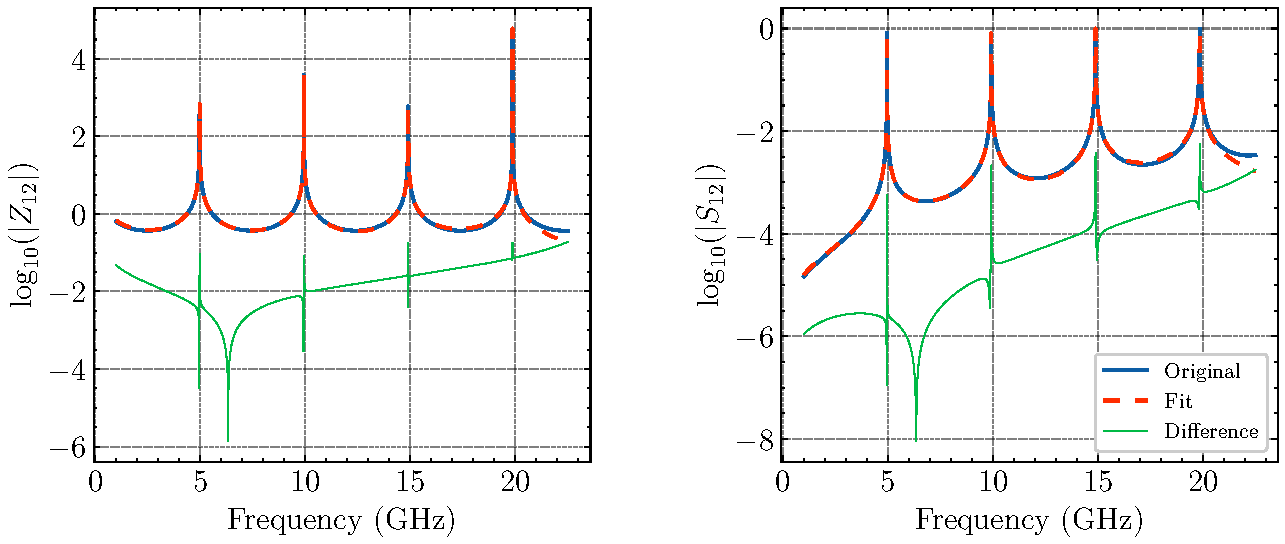
\includegraphics[width=\textwidth]{figures/ideal_TL_fit.pdf}
    \caption{Fit results for the off-diagonal elements of the impedance and scattering parameters for the two-port network in Fig.\ \ref{fig:ideal_TL_coupler}. The diagonal elements of the parameters show similar or smaller difference. For the capacitors we choose $C_1 =$ 70 fF, $C_2 =$ 72 fF, $C_{1c}=C_{2c} =$ 6.5 fF. For the transmission line we choose $L = $ 0.438 $\mu$H/m, $C = $ 0.159 nF/m, $\ell =$ 12 mm.}
    \label{fig:ideal_TL_coupler_fit}
\end{figure}

Using the fitted rational impedance function, we can write out the Hamiltonian of the system using (\ref{eq:impedance_hamiltonian}) once we've taken into account the Josephson junctions at the ports. With both transmons at $\omega_1/2\pi=\omega_2/2\pi = $ 4 GHz, they have a direct coupling rate of $g_{12} = 0.652$ MHz. The coupling rates of the transmons to the resonant modes are shown in Table \ref{table:ideal_TL_coupling}.

\renewcommand{\arraystretch}{1.5}
\begin{table}[h!]
    \centering
    \begin{tabular}{|r|r|r|r|r|}
    \hline
    $\omega_{R_k}/2\pi$ (GHz) & $4.965470$   & $9.931947$   & $14.896434$  & $19.8619404$ \\ \hline
    $g_{1,R_k}/2\pi$ (MHz)   & $-55.113$ & $-77.924$ & $-95.422$ & $-110.154$ \\ \hline
    $g_{2,R_k}/2\pi$ (MHz)   & $54.367$  & $-76.869$ & $94.130$  & $-108.662$ \\ \hline
\end{tabular}
\caption{The resonant pole positions $\omega_{R_k}$ from the fit result in Fig.\ \ref{fig:ideal_TL_coupler_fit} and their corresponding coupling rates to the transmons.}
\label{table:ideal_TL_coupling}
\end{table}
\renewcommand{\arraystretch}{1}

Using the resulting Hamiltonian, we can construct the effective Hamiltonian for the system that only contains the transmons. Then we can simulate the time evolution of the full Hamiltonian (\ref{eq:transmon_resonator_ham}) containing the four resonant modes and compare it to the simulation of the effective Hamiltonian (\ref{eq:eff_ham}). An example showing agreement between the two is shown in Fig.\ \ref{fig:ideal_TL_coupler_sim}.

\begin{figure}[!h]
    \centering
    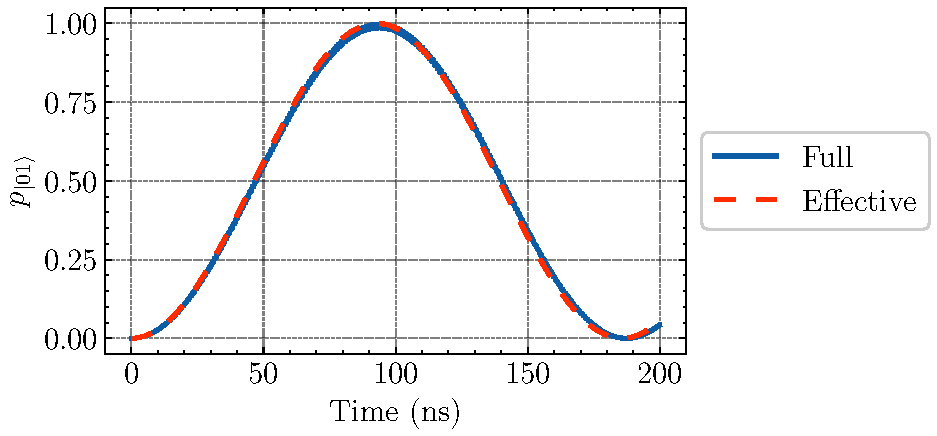
\includegraphics[width=0.6\textwidth]{figures/ideal_TL_sim.pdf}
    \caption{Time evolution of the full and effective Hamiltonians for the circuit in Fig.\ \ref{fig:ideal_TL_coupler} using the results from the fit in Fig.\ \ref{fig:ideal_TL_coupler_fit}. The transmons are at 4 GHz and the initial state is $\ket{Q_1Q_2}=\ket{10}$ with all the resonators of the full Hamiltonian in the ground state.}
    \label{fig:ideal_TL_coupler_sim}
\end{figure}

Using the same circuit, we can look at what happens to our estimate of the effective coupling rate between the qubits when we increase the cutoff frequency used for our fit. When increasing this range, more resonances are visible in the response and are then included as new resonance modes in the fitted rational impedance. We start by fitting a function that includes just the first resonant mode. Then for each of the next highest resonant modes, we fit new functions until we have reached a total of 40 resonant modes included. Note that this is only performed as a test of the fitting process and to see how the effective coupling formulas are affected by including these higher resonant modes. The fit for the frequency range that contains 40 resonant modes is shown in Fig.\ \ref{fig:ideal_TL_coupler_fit_40_res}. The fitting for this wide frequency range is quick (less than 30 seconds) and the results here only use the lossless part of the impedance obtained from the traditional vector fitting process.

\begin{figure}[!h]
    \centering
    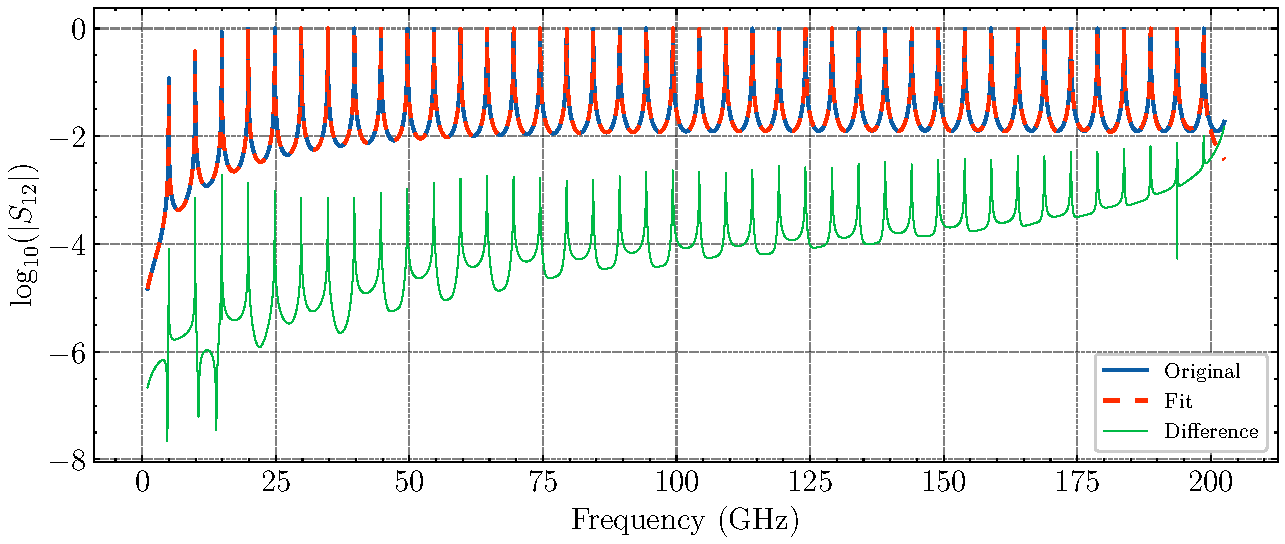
\includegraphics[width=\textwidth]{figures/ideal_TL_fit_40_res.pdf}
    \caption{Fit results for the $S_{12}$ parameter for the two-port network in Fig.\ \ref{fig:ideal_TL_coupler}. Here, 40 resonant modes are included in the frequency range.}
    \label{fig:ideal_TL_coupler_fit_40_res}
\end{figure}

\begin{figure}[!h]
    \centering
    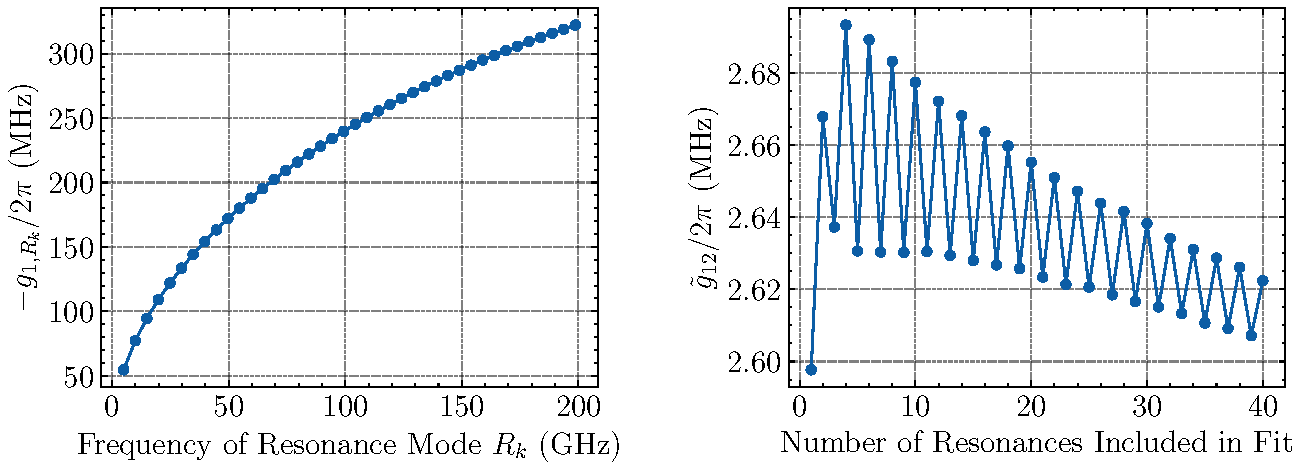
\includegraphics[width=\textwidth]{figures/ideal_TL_coupling_change.pdf}
    \caption{Left: For the fitted network in Fig.\ \ref{fig:ideal_TL_coupler_fit_40_res}, the coupling $g_{1,R_k}$ is shown for all 40 resonant modes present in the fit. Right: Effective coupling estimate (\ref{eq:eff_qubit_coupling}) as a function of the number of resonances included in the fit of the impedance function. Transmon frequencies are $\omega_1/2\pi=\omega_2/2\pi = $ 4 GHz.}
    \label{fig:ideal_TL_geff_change}
\end{figure}

First, we see that the coupling between the resonant modes and the transmons diverge as the resonant modes goes to higher frequency ($g_{i,R_k} \propto \omega_{R_k}^{1/2}$). This divergence is expected given that the Hamiltonian (\ref{eq:transmon_hamiltonian}) that we start with cannot account for the infinite number of resonant modes introduced by the ideal transmission line \cite{Parra-Rodriguez_2018}. This has the effect that the estimate of the effective coupling will also diverge if continuing to include higher resonant modes. In the effective coupling there is also an oscillation due to the alternating signs present in the coupling of one of the transmons to the resonant modes. This can be seen clearly in Table \ref{table:ideal_TL_coupling} and also in a similar example in Appendix \ref{appendix:cascade_ideal_TL}. In reality, there is a natural cutoff frequency for these resonant modes that is dependent on the superconducting gap frequency. In addition, there will be higher loss or attenuation in the material at higher frequencies that will reduce the coupling through the higher resonant modes \cite{picosecond_pulses,harmonic_superconducting}. These factors can help in choosing the cutoff frequency for our fitting.